\presec
\section{Related Work} \postsec
\label{sec:relatedwork}

In this section, we first show the differences between PRI and USS. Second, we show the related work in finding heavy changes, Super-Spreaders, and persistent items. The related work in finding frequent items has been presented in Section \ref{sec:intro:priorart}.

{\color{reviewC}
\subsection{Differences Between PRI and USS}

We summarize the nine differences between PRI and USS, and we give two examples to illustrate these differences.

\ppp{Definitions:} let $e_{min}$ be the smallest item, $I_{min}$ be $e_{min}$'s interest, and $t_{fail}$ be the number of failed replacements.

\ppp{Difference1:} $P_{pri} = \frac{1}{2I_{min} - t_{fail}+1}$, while 
$P_{uss} = \frac{1}{I_{min}+1}$.

\ppp{Difference2:} When the replacement is failed, 1) PRI: $t_{fail}++$, $I_{min}$ does not change, thus $P_{pri}$ increases; 2) USS: $I_{min}++$, thus $P_{uss}$ decreases. 

\ppp{Difference3:} When the replacement is successful, 1) PRI: $I_{min} += \frac{t_{fail}}{I_{min}}$, $t_{fail}=0$; 2) USS: $I_{min} ++$. 

\ppp{Difference4:} PRI increases $I_{min}$ only after a successful replacement. USS increases $I_{min}$ by 1 for each new incoming item, incurring significant overestimation. 


\ppp{Difference5:} To successfully replace $e_{min}$, 
1) PRI: the expectation of $t_{fail}$ is $I_{min}$. PRI needs in average $I_{min}+1$ items to successfully replace $e_{min}$. 2) USS: the expectation of $t_{fail}=\sum_{i=0}^{\infty}\frac{x(i+1)}{(x+i)(x+i+1)}$, which does not converge. 


\ppp{Difference6:} When $t_{fail}$ reaches $2I_{min}$: 1) $P_{pri}$ increases to 1, avoiding too many replacement failures; 2) $P_{uss}$ decreases to $1/(3I_{min}+1)$. 


\ppp{Difference7:} 1) USS is unbiased, for it assumes all other items not recorded have a frequency of 0, i.e., the recorded items are drastically overestimated. 2) PRI: each recorded item is accurate. 

\ppp{Difference8:} 1) USS inherits the SpaceSaving's data structure: Stream-Summary, which is memory consuming. 2) Final version of PRI: storing multiple items in one bucket, which is memory efficient. 


\ppp{Difference9:} 1) USS is used for only heavy hitters;
2) PRI is used for 4 interests.


Below We also give two examples to compare the performance of USS and PRI. 

\ppp{Example1:} We use one bucket to find the largest item. Assume item A arrives 10 times, then B arrives 10 times. 
\par
\noindent 1) USS: $<B,20>$ with a probability of 1/2, or $<A,20>$ with a probability of 1/2. Average Relative Error(ARE) is 1. \par
\noindent 2) PRI: probability of $<A,10>$ is 11/21 and that of $<B,10>$ is 1/21, which have no error. ARE is 0.21. 


\ppp{Example2:} Similarly, assume there are $10^6$ distinct items, each of which arrives 10 times. \par
\noindent 1) USS: ARE is $10^6-1$. \par
\noindent 2) PRI: ARE is in average 947 according to our test results. 947 is 1000 times smaller than $10^6-1$, which is consistent with our experimental results.
Our final version stores multiple items in one bucket instead of Stream-Summary, further decreasing ARE.
}

%\ppp{2) Finding Heavy Changes:}
%Here, a data stream is equally divided into $n$ periods (also known as time windows or intervals). We define interest as \textit{change of frequency}, \ie, the difference of frequency of an item in two adjacent periods.
%
%Again, the first type of solution is to \texttt{record all}, including k-ary \cite{kary}, the reversible sketch \cite{revsketch}, and FlowRadar \cite{flowradar}. 
%They build one data structure to record all items in each period, and then manage to decode and report heavy changes. 
%
%The second kind manages to record only hot items, and the typical algorithm being Cold filter \cite{coldfilter}.
%Cold filter first uses a filter to filter cold items, and then focuses on hot items. We aim to achieve a higher accuracy than Cold filter without any additional data structure.


%\ppp{3) Finding Super-Spreaders:}
%Each item is a packet with a source IP address and a destination IP address. We define interest as \textit{connections}, \ie, the number of destination IP addresses for a given source IP address. The problem is to find source IP addresses with large number of connections.
%
%Again, two kinds of solutions exist. The first, \texttt{record all}, records the information of all packets. Typical algorithms are Two-dimension bitmap \cite{twodimensional} and OpenSketch \cite{opensketch}. 
%The second kind, \texttt{record samples}, samples packets before recording the information of packets. Sampling achieves memory efficiency at the cost of poor accuracy.
%The typical algorithms here are called one-level filtering \cite{superspreader} and two-level filtering \cite{superspreader}. We aim to record only Super-Spreaders without sampling, to achieve a higher accuracy. 

%\ppp{4) Finding Persistent Items:}
%Here, a data stream is equally divided into $n$ periods. 
%
%We define interest as \textit{persistency}, \ie, the number of periods in which the item appears.
%
%In each period of the stream, the persistency of an item is incremented only once or not changed. 
%
%The problem is to find items with high persistency.
%
%Again, two types of solutions exist. The first, \texttt{record all}, records the information of all packets. The typical algorithm is PIE \cite{persisitem}. The second kind, \texttt{record samples}, samples before recording the information of items. The typical algorithm is small-space \cite{smallspace}. 
%
%We aim to record only persistent items to achieve a higher accuracy. 

%In contrast, we aim to design a generic framework, which can be used for finding any interesting items with high speed and high accuracy at the same time.
%\presub 
\begin{comment}

\subsection{Prior Art for Finding Frequent Items} \postsub

To find frequent items, as mentioned above, existing solutions can be divided into two kinds.
%
The first kind is called \texttt{record all}, which records the information of all items. 
This kind uses a sketch plus a min-heap or an array.
Typically, we can use sketches of CM \cite{cmsketch}, CU \cite{cusketch}, and Count\cite{countsketch}.
%
Since the three sketches are similar to a large extent, we only introduce the CM sketch, as it is the most widely used. In a CM sketch, there are $d$ arrays corresponding to $d$ hash functions. For an incoming item, it first calculates $d$ hash functions and gets $d$ hashed counters, each of which is incremented by one. When reporting the frequency of a specific item, the $d$ hash functions of the ID are first calculated and the smallest hashed counter is returned. When inserting an item, if its estimated frequency is larger than the smallest frequency in the min-heap, the item is inserted into the min-heap.
%
A sophisticate sketch, ASketch \cite{asketch}, uses a small filter acting as a cache to capture hot items, and records other items in a CM sketch, achieving higher speed and accuracy than only using a CM sketch. The authors recommend storing only 32 hot items in the filter, and thus ASketch focuses on frequency estimation rather than frequent items. 
%ASketch~\cite{asketch} aims at optimizing the accuracy by using a small array instead of the min-heap. The array acts like a cache for the hottest items. The caching process involves exchanges between the sketch and the array. The items in the array that are never exchanged have no error. 
%
%However, the array is very small, and the authors recommend storing only 32 items in the array, and therefore ASketch mainly focus on frequency estimation ra.
%

%Typical algorithms are a sketch (\eg, sketches of CM \cite{cmsketch}, CU\cite{cusketch}, and Count \cite{countsketch}) plus a min-heap, and ASketch \cite{asketch}. 
%


Realizing that it is unnecessary and harmful to record frequencies of cold items, the idea of the second kind of solution, \texttt{record part}, records the information of only hot items.
%
For this kind of solution, the most well-known algorithm is SpaceSaving \cite{spacesaving}. 
It has various variants: the Unbiased SpaceSaving \cite{unbiasedsketch}, Cold filter, and more \cite{css}.
The key operation of SpaceSaving is as follows. It uses a min-heap-like data structure -- Stream-Summary. When a new item $e$ arrives, it increments the smallest frequency $f_{min}$ in Stream-Summary by 1, and then replaces the smallest item with $e$.
%
SpaceSaving has only over-estimation error.
%
Based on SpaceSaving, the Unbiased SpaceSaving \cite{unbiasedsketch} makes a small modification: when a new item $e$ arrives, it also increments the smallest frequency $f_{min}$ by 1, but then replaces the smallest item with $e$ with a probability.
%
The Unbiased SpaceSaving is proved theoretically to be unbiased.
%
For SpaceSaving and the Unbiased SpaceSaving, every cold item will increment the smallest frequency, and since most items are cold in practice, leads to poor accuracy.
%
Noticing the negative effect of cold items, Cold filter \cite{coldfilter} filters cold items using a small CU sketch, achieving a much higher accuracy.
%
In contrast, we aim to minimize the negative effect above with no auxiliary data structures.
\end{comment}

\vvv
\presec
\subsection{Prior Art for Finding Heavy Changes}\postsec~
\hl{
In finding heavy changes, a data stream is equally divided into $n$ periods (also known as time windows or intervals). In this task, interest is defined as \textit{change of frequency}, i.e., the difference of frequency of an item in two adjacent periods.
}

%Again, the first type of solution is to \texttt{record all}, including k-ary \cite{kary}, the reversible sketch \cite{revsketch}, and FlowRadar \cite{flowradar}. 
%The second kind manages to record only hot items, and the typical algorithm being Cold filter \cite{coldfilter}.
%Cold filter first uses a filter to filter cold items, and then focuses on hot items. We aim to achieve a higher accuracy than Cold filter without any additional data structure.

To find heavy changes, there are also two kinds of algorithms.
%
The first kind is \texttt{record all}, recording the information of all items.
\hl{They build one data structure to record all items in each period, and then manage to decode and report heavy changes.} Typical algorithms include k-ary \cite{kary}, the reversible sketch \cite{revsketch}, and FlowRadar \cite{flowradar}. 
%
The k-ary sketch \cite{kary} can only record the difference of frequencies, but cannot record item IDs.
%
To overcome this shortcoming, the reversible sketch \cite{revsketch} improves the k-ary sketch by estimating the item IDs with time complexity of $O(2^{0.75\text{L}})$ (L is the number of bits of item ID), which can be very large. 
FlowRadar \cite{flowradar} uses a Bloom filter to remove duplicates, and records each item in a modified Invertible Bloom Lookup Table (IBLT) \cite{iblt}. The time complexity to decode item ID is $O(n)$ ($n$ is the number of distinct items). When IBLT uses the appropriate parameters, FlowRadar can successfully decode all the items with high probability. As FlowRadar records and decodes all items, it is not memory efficient. 
%
The second kind of solutions manages to record only the hot items, and the typical algorithm is Cold filter \cite{coldfilter}. Based on FlowRadar, Cold filter \cite{coldfilter} uses an additional filter to filter cold items, and only inserts hot items into FlowRadar, thus achieving a higher accuracy.
%
However, as FlowRadar is inherently not a compact data structure, it is still not memory efficient despite using Cold filter.

\begin{figure*}[!ht]
	\centering
	%
	\subfigure[Synthetic dataset]{
		\begin{minipage}[t]{0.255\textwidth}{
		\prefig
		\begin{center}
		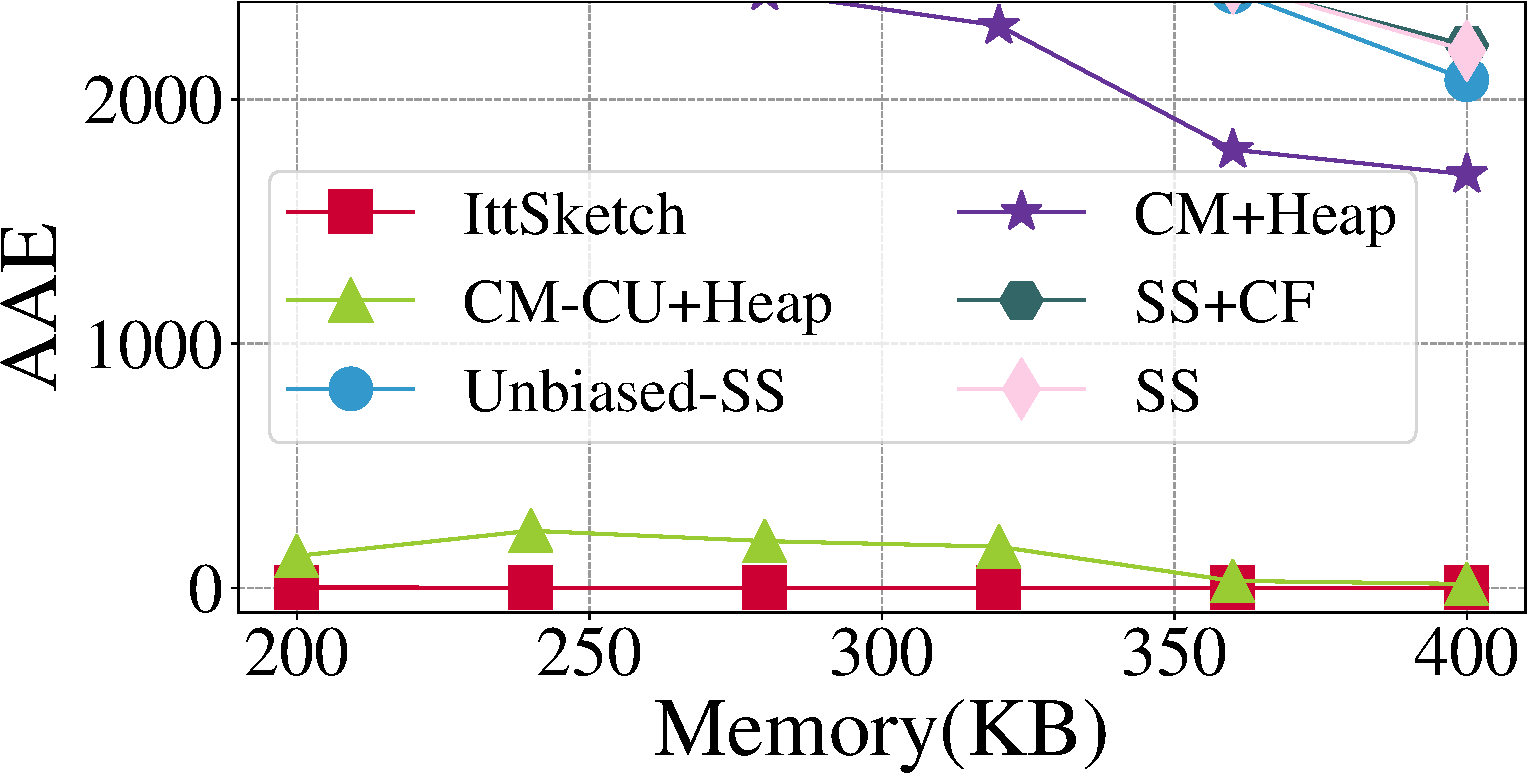
\includegraphics[width=0.95\textwidth, ]{Figures/fre/fre_aae/fre_syn_aae-cropped.pdf}
		\end{center}
	    }
		\postfig
		\adjustfigs
		\prefigcaption
		\label{fre_aae_syn}
		\postfigcaption
		\end{minipage}
	}
    %
	\subfigure[IP trace]{
		\begin{minipage}[t]{0.225\textwidth}{
		\prefig
		\begin{center}
		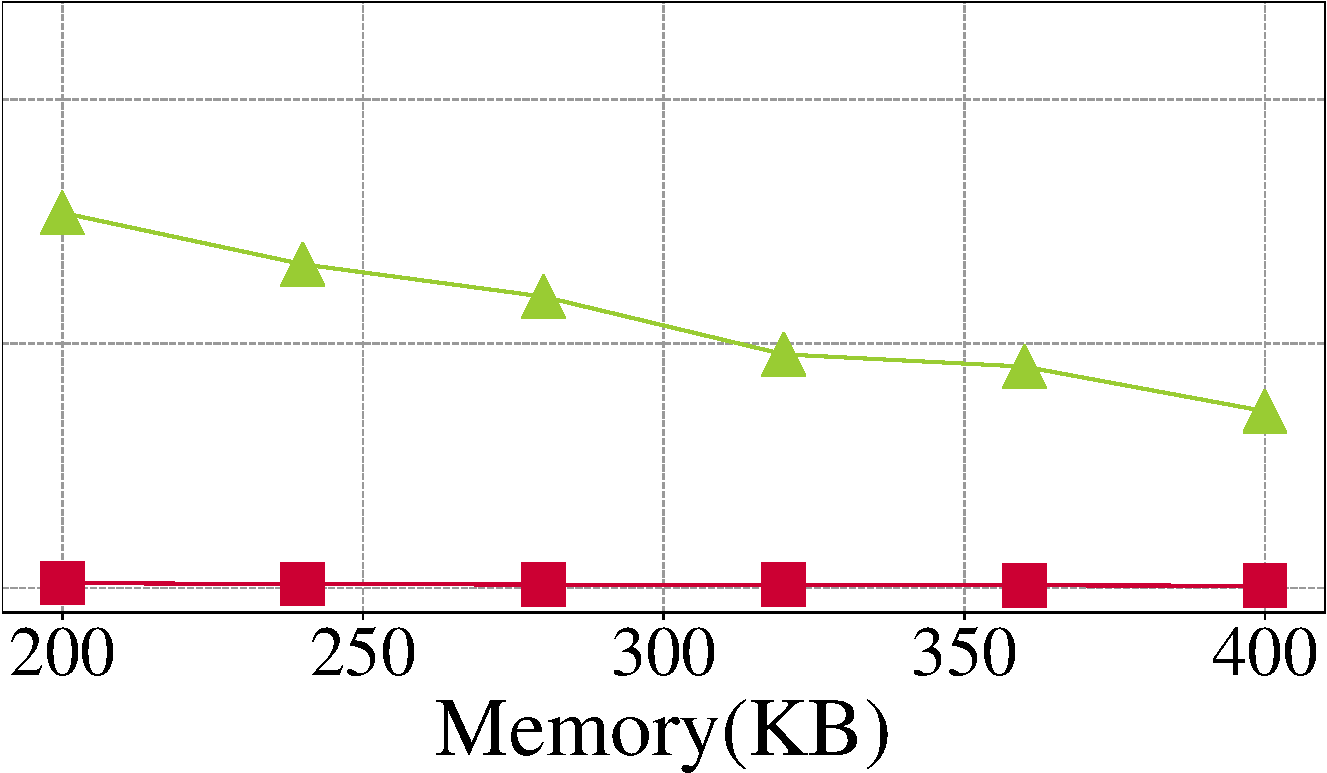
\includegraphics[width=0.95\textwidth, ]{Figures/fre/fre_aae/fre_ip_aae-cropped.pdf}
		\end{center}
		}
		\postfig
		\adjustfigs
		\prefigcaption
		\label{fre_aae_ip}
		\postfigcaption
		\end{minipage}
	}
    %
	\subfigure[Web page]{
		\begin{minipage}[t]{0.225\textwidth}{
		\prefig
		\begin{center}		
		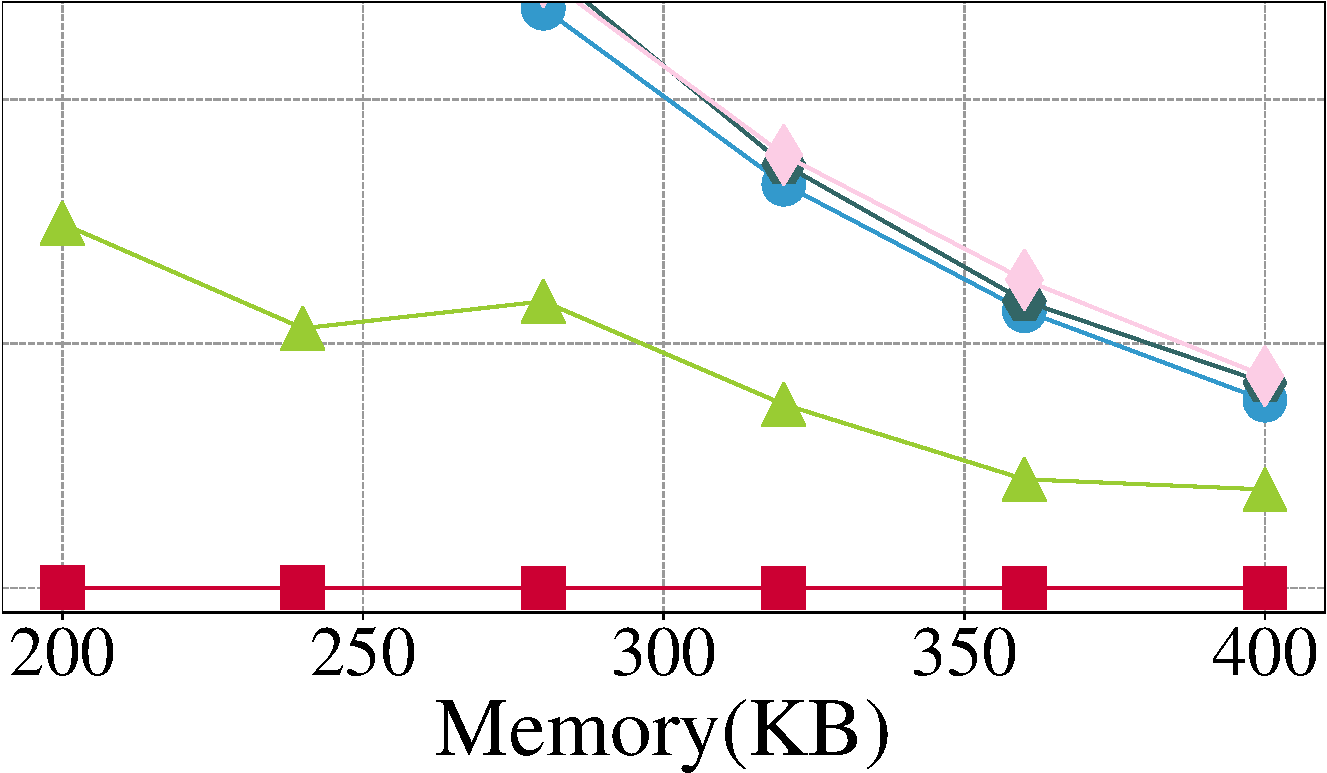
\includegraphics[width=0.95\textwidth]{Figures/fre/fre_aae/fre_web_aae-cropped.pdf}
		\end{center}
		}
		\postfig
		\adjustfigs
		\prefigcaption
		\label{fre_aae_web}
		\postfigcaption
		\end{minipage}
	}
	%
	\subfigure[Network dataset]{
		\begin{minipage}[t]{0.225\textwidth}{
		\prefig
		\begin{center}		
		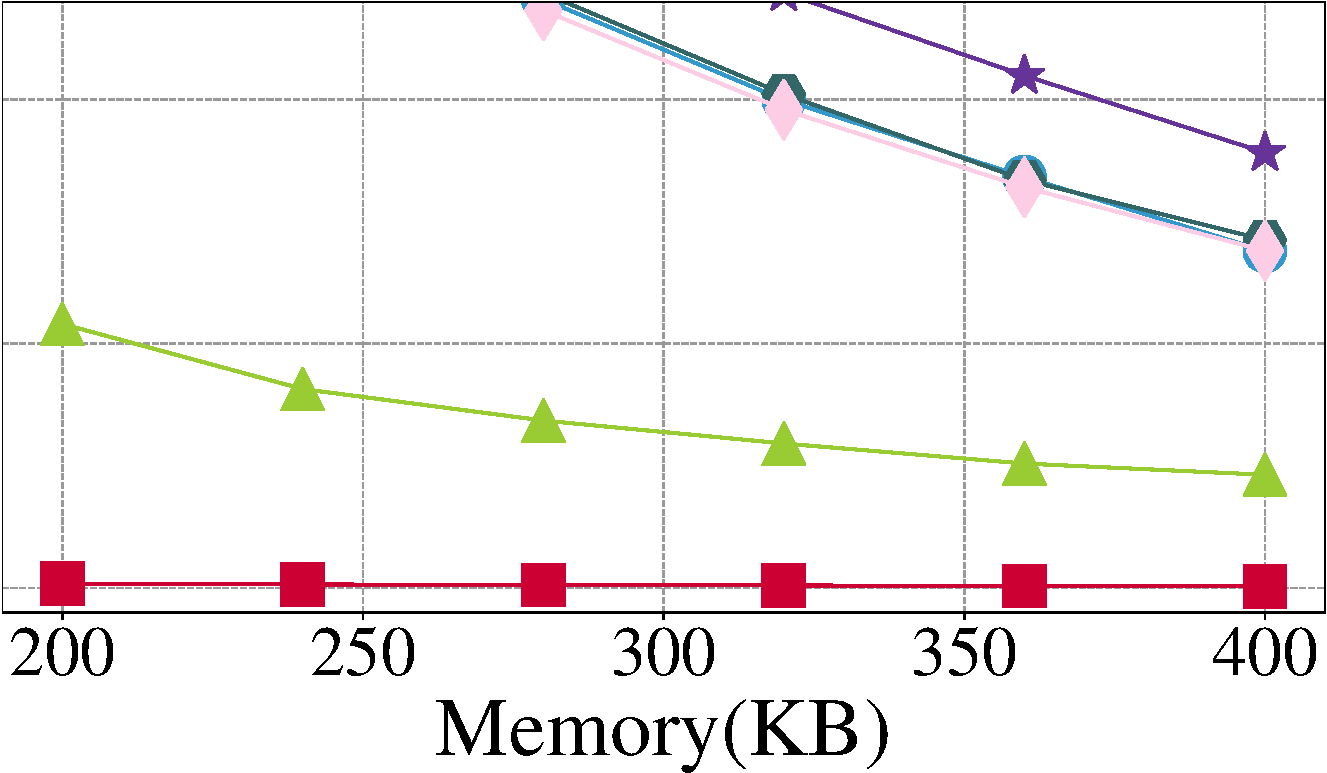
\includegraphics[width=0.95\textwidth]{Figures/fre/fre_aae/fre_net_aae-cropped.pdf}
		\end{center}
		}
		\postfig 
		\adjustfigs
		\prefigcaption
		\label{fre_aae_net}
		\postfigcaption
		\end{minipage}
	}
	%
	\vvv \vvv
	\caption{AAE of finding \taskone.}
	\label{fre_aae}
\end{figure*}
			
\begin{figure*}[!ht]
	\centering
	%
	\subfigure[Synthetic dataset]{
		\begin{minipage}[t]{0.255\textwidth}{
		\prefig
		\begin{center}
		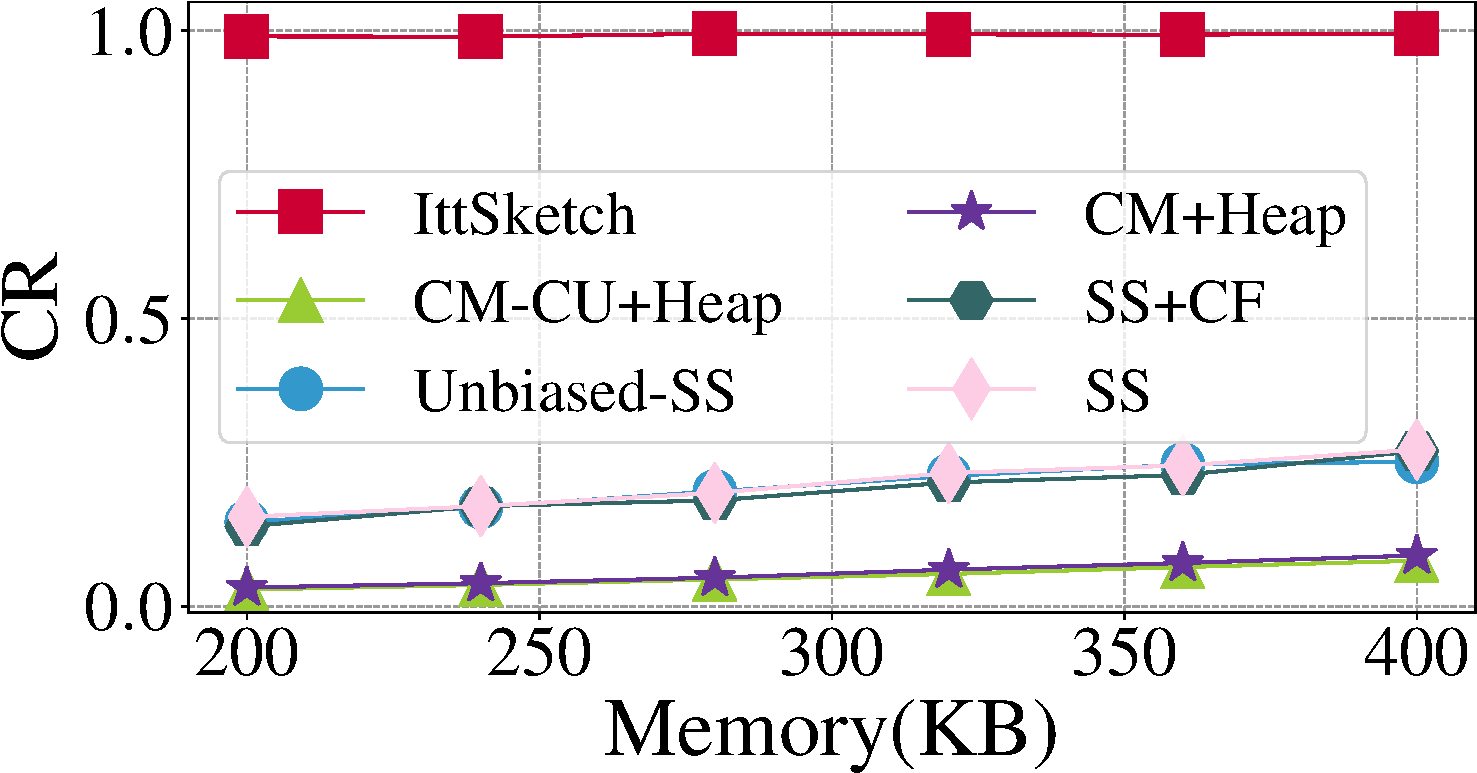
\includegraphics[width=0.95\textwidth, ]{Figures/fre/fre_cr/fre_syn_cr-cropped.pdf}
		\end{center}
		}
		\postfig 
		\adjustfigs
		\prefigcaption
		\label{fre_cr_syn}
		\postfigcaption
		\end{minipage}
	}
	%
	\subfigure[IP trace]{
		\begin{minipage}[t]{0.23\textwidth}{
		\prefig
		\begin{center}
		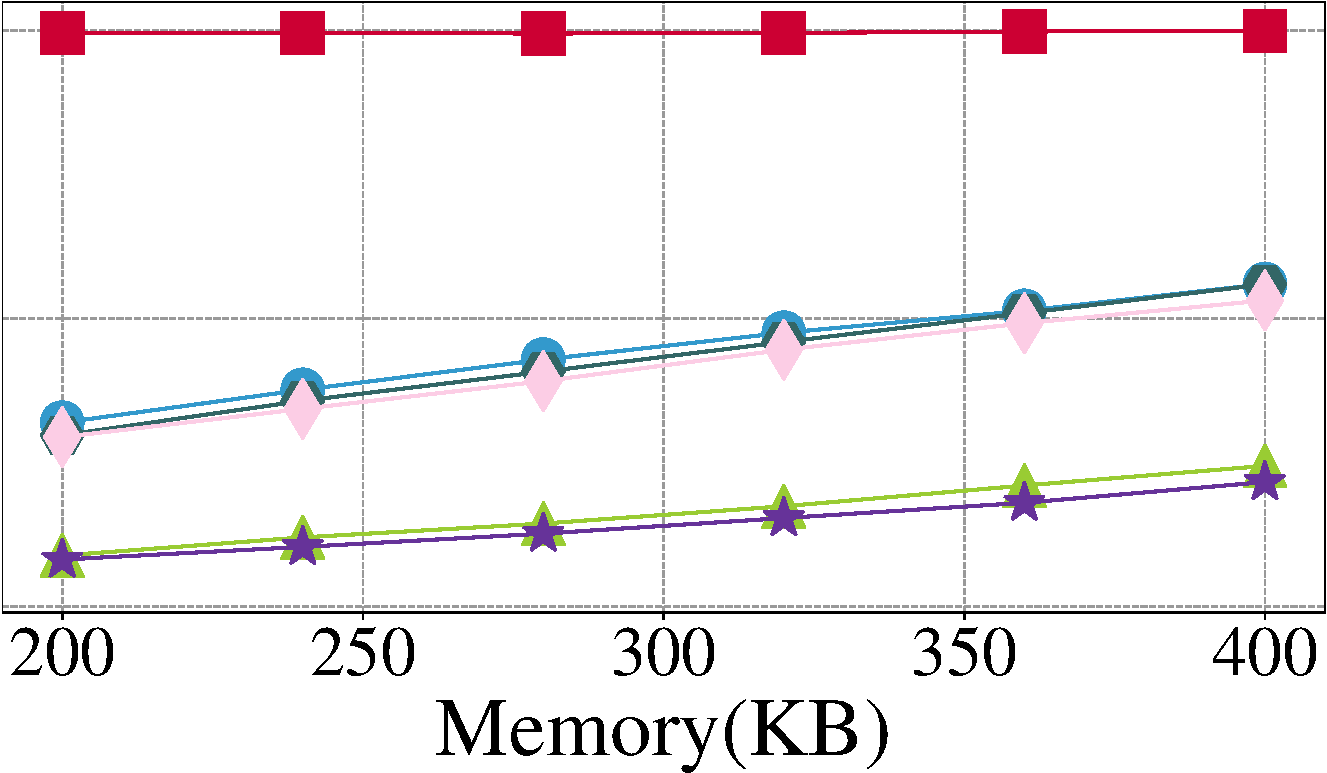
\includegraphics[width=0.95\textwidth, ]{Figures/fre/fre_cr/fre_ip_cr-cropped.pdf}
		\end{center}
		}
		\postfig
		\adjustfigs
		\prefigcaption
		\label{fre_cr_ip}
		\postfigcaption
		\end{minipage}
	}
	%
	\subfigure[Web page]{
		\begin{minipage}[t]{0.23\textwidth}{
		\prefig
		\begin{center}		
		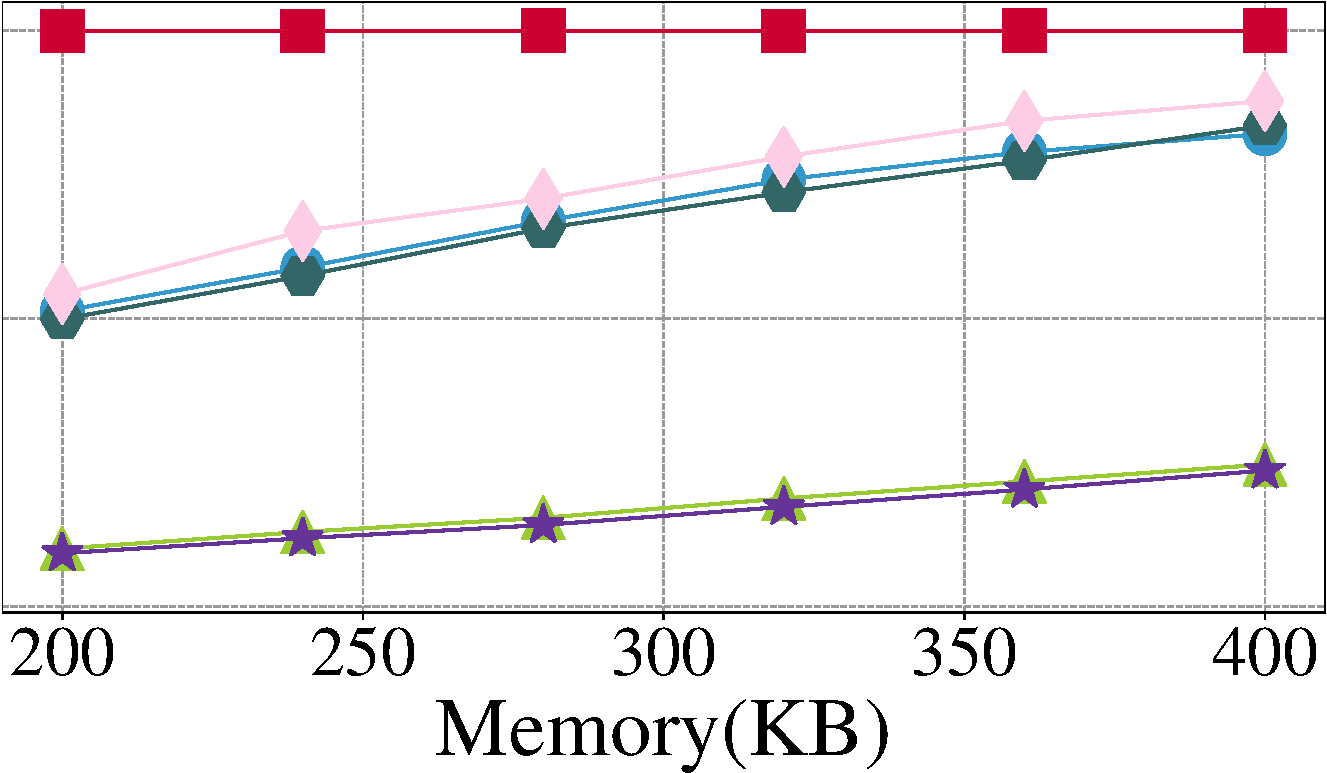
\includegraphics[width=0.95\textwidth, ]{Figures/fre/fre_cr/fre_web_cr-cropped.pdf}
		\end{center}
		}
		\postfig 
		\adjustfigs
		\prefigcaption
		\label{fre_cr_web}
		\postfigcaption
		\end{minipage}
	}
	%
	\subfigure[Network dataset]{
		\begin{minipage}[t]{0.23\textwidth}{
		\prefig
		\begin{center}		
		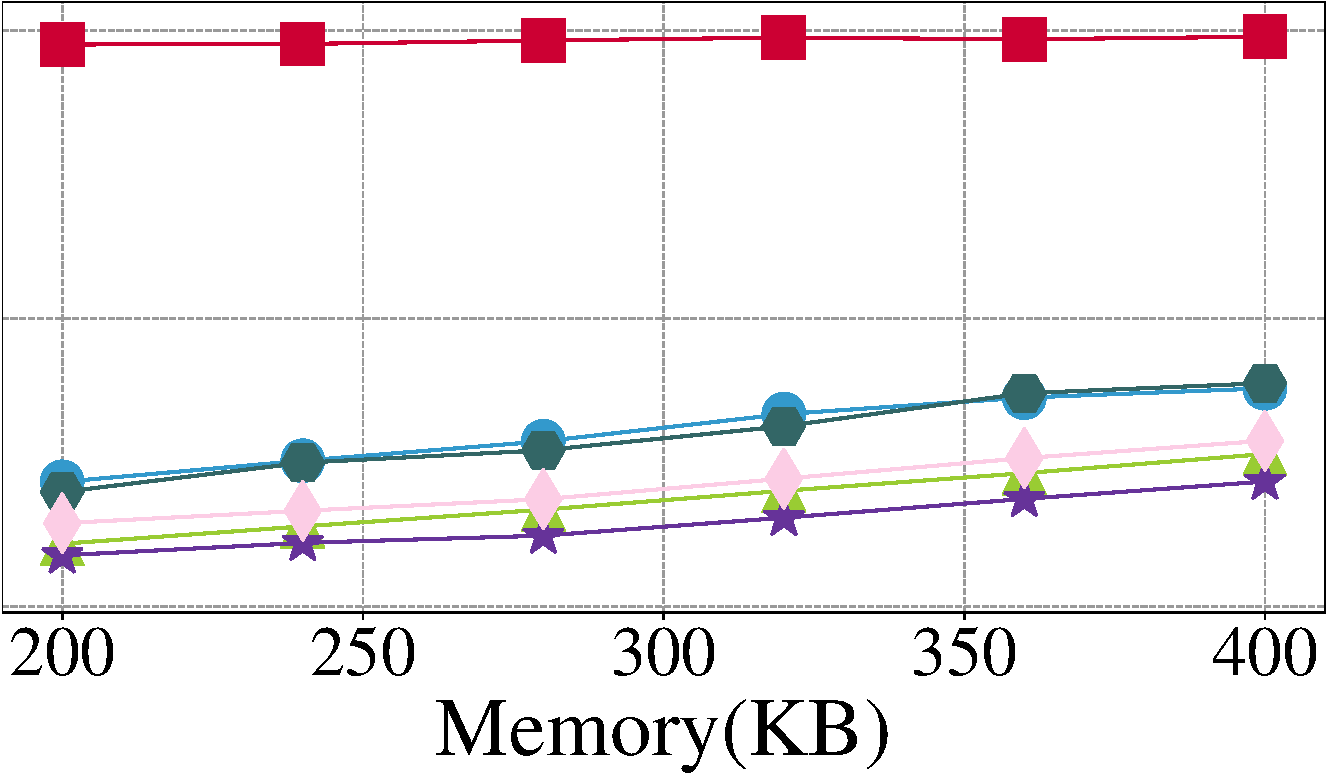
\includegraphics[width=0.95\textwidth, ]{Figures/fre/fre_cr/fre_net_cr-cropped.pdf}
		\end{center}
		}
		\postfig 
		\adjustfigs
		\prefigcaption
		\label{fre_cr_net}
		\postfigcaption
		\end{minipage}
	}
	%
	\vvv \vvv
	\caption{CR of finding \taskone.}
	\label{fre_cr}
\end{figure*}

\vvv
\presec
\subsection{Prior Art for Finding Super-Spreaders}\postsec~
%Each item is a packet with a source IP address and a destination IP address. 
%We define interest as \textit{connection}
%\ie, 
%the number of destination IP addresses for a source IP address. 
%The problem will be finding source IP addresses with large connections.
%
%Super-Spreader refers to those source IP addresses with the largest connections. 
\hl{
In finding Super-Spreaders, each item is a packet with a source IP address and a destination IP address. Interest is defined as \textit{connections}, i.e., the number of destination IP addresses for a given source IP address. This problem is to find source IP addresses with large number of connections.}

Again, there are two kinds of solutions for finding Super-Spreaders. 
The first is \texttt{record all}, which records the information of all packets. Typical algorithms are Two-dimension bitmap \cite{twodimensional} and OpenSketch \cite{opensketch}. 
%
Two-dimension bitmap \cite{twodimensional} uses a matrix of bits. To insert a packet, the source IP address is hashed to a row of the matrix while the destination IP address is hashed to a column. Then a bit is located and set to 1.
%
For a source IP address, the number of 1s in the mapped row can be used to estimate the number of connections. By adding a min-heap, Super-Spreaders can be found.
%
As the number of Super-Spreaders are often small, most rows are empty, which is a waste of memory.
%
To find Super-Spreaders, OpenSketch \cite{opensketch} combines the techniques of CM sketches (presented above) and bitmaps. It replaces each counter in the CM sketch by a bitmap. The number of 1s in each bitmap is used to estimate the number of connections. 
%
The bitmap needs to be large enough to accurately estimate the connections. Therefore, OpenSketch is accurate when using large amounts of memory.

The second kind is again \texttt{record samples}.
As there are many items, even simple sampling can automatically filter/discard many cold items, saving memory.
The typical algorithms are called one-level filtering \cite{superspreader} and two-level filtering \cite{superspreader}. Besides sampling, they remove duplicates by using a hash function.
%
Specifically, given an incoming packet $e$, they hash the combination of source and destination IP into the range [0, 1]. If the hash value is larger than the given threshold, $e$ is chosen; otherwise, $e$ is discarded.
Then, it uses a hash table to record all samples before it reports Super-Spreaders.
%
Indeed, sampling can save memory, but the incurred error is hard to reduce.
%
Our method on the other hand can achieve a higher accuracy, and can be used together with the sampling method.
%which samples before recording the information of packets. 
%Our algorithm tries to record only super-spreaders, thus can achieve much higher accuracy. 

\vvv
\presec
\subsection{Prior Art for Finding Persistent Items}\postsec~
\hl{In find persistent items, a data stream is equally divided into $n$ periods. Interest is defined as \textit{persistency}, i.e., the number of periods in which the item appears. In each period of the stream, the persistency of an item is incremented only once or not changed. The problem is to find items with high persistency.}

Again, two types of solutions exist to find persistent items. The first, \texttt{record all}, records all packets. The typical algorithm is PIE \cite{persisitem}. 
%
For each time period, PIE uses a hash table to record the incoming items fingerprints. When a collision happens, the fingerprint is set to invalid.
%
The key technique is to use Raptor codes \cite{raptorcode} to generate different fingerprints in different periods.
%
For a persistent item occurring in many periods, many valid fingerprints can be found, and these can be used to recover the item ID.
%
Therefore, persistent items have a higher probability to be successfully recovered.
%
However, due to the recording of cold items and collisions, the accuracy of PIE is not high.

The second kind, \texttt{record samples}, samples and removes duplicates before recording packets. 
%
The typical algorithm is called small-space \cite{smallspace}. 
%
As mentioned earlier, sampling can save memory.
%
The algorithm of small-space is similar to one-level filtering \cite{superspreader}.
%
The only difference is that it 
hashes the item ID plus the index of period for removing duplicates.
%
Our method can achieve a higher accuracy, and can be used together with the sampling method.

\presub
\subsection{Other Sketches} \postsub
Except for the above four tasks, sketch techniques also attract the attention of researchers in other applications. 
Due to space limitation, here we only list them: TCM \cite{tang2016graph}, SVS \cite{SVS},
DA2 \cite{DA}, bias-aware sketches \cite{bias-aware-sketch}, Ada-sketches \cite{ada-sketch}, SuRF \cite{surf}, Counting Quotient Filter \cite{general-purpose-counting-filter},
Persistent Bloom filters \cite{persistent-bf}, SketchML \cite{sketchml}, and more \cite{wmsketch, cormode2011synopses}.

\section{Experimental Figures on AAE and CR}
\label{app:fig}
Due to space limitation, we show the experimental figures on AAE and CR here (see Figure~\ref{fre_aae}-\ref{per_cr}), and we observe the similar results and get similar conclusions.

\begin{comment}
Here we give a brief overview of recent works. Interested readers please refer to the excellent book \cite{cormode2011synopses}.

TCM \cite{tang2016graph} is a sketch for graph streams, which supports a wide range of graph queries. 
SVS \cite{SVS} is an algorithm to output a covariance sketch over massive distributed data metrics.
DA2 \cite{DA} is another algorithm to track covariance sketch over distributed sliding windows.

For the task of frequency estimation, bias-aware sketches \cite{bias-aware-sketch} outperforms other sketches when there is a bias in the frequency vector of the data stream.
Ada-sketches \cite{ada-sketch} supports queries by time ranges as well as time points, and provide better accuracy for queries on recent time than that on old time. 
For membership query, SuRF \cite{surf} supports approximate range membership query, besides the point query which is supported by most filters. Counting Quotient Filter \cite{general-purpose-counting-filter} is designed to  support deletion and counting, and has good data locality on SSDs. Persistent Bloom filters \cite{persistent-bf} can be used for temporal membership queries.
Sketches can also be used in machine learning.
SketchML \cite{sketchml} tries to use sketches to compress the gradients exchanged in the network, so as to reduce the training time.
The authors in \cite{wmsketch} use a sketch to express the model of the linear classifier, to support model training on memory-limited devices.
\end{comment}



